\documentclass[11pt]{article}
\usepackage[final]{acl}
\usepackage{times}
\usepackage{latexsym}
\usepackage[T1]{fontenc}
\usepackage[utf8]{inputenc}
\usepackage{microtype}
\usepackage{graphicx}
\usepackage{booktabs}
\usepackage{amsmath}
\usepackage{tabularx}
\usepackage{xcolor}
\usepackage{balance}
\setlength{\emergencystretch}{1.5em}
\raggedbottom
\graphicspath{{../figures/}}
\title{Reproducing VADER and Testing Sentiment Robustness\\on New Short Text Data}
\author{COMP8240: Applications of Data Science\\Assessment 3: Project Final Report\\4 November 2026}
\date{}

\begin{document}
\maketitle
\begin{abstract}
This project examines the reproducibility and transfer of VADER using its released
evaluation resources, a newer sentiment benchmark, and controlled short texts.
Both an archived implementation and a maintained implementation were executed on
all 23,703 original evaluation texts. The archived version reproduces the published
tweet-like and editorial correlations to three decimal places; movie and product
correlations differ. A classification audit shows substantial sensitivity to the
conversion of human intensity ratings and the averaging convention for F1.
On DynaSent, archived macro-F1 is 0.549 on the 3,600-item Round 1 test set and
0.523 on the 720-item Round 2 test set. Maintained code produces very similar
results, with paired confidence intervals spanning zero for its improvement.
A new 288-text diagnostic corpus covers negation, modification, capitals,
punctuation and contrast. Its score changes expose lexical coverage failures,
but independent human validation remains incomplete. A preserved within-session
assistant-judge pilot is reported separately from human reference evidence.
The completed experiments support partial replication and limited transfer,
with explicit boundaries on the claims that the constructed data can support.
\end{abstract}

\noindent\textbf{Review-draft status.} Independent human annotation of the
constructed corpus and verification of the student's public project repository
remain pending. No human ratings, consent records, or annotation agreement
statistics have been invented. The accompanying source package records completed
experiments and the exact remaining dependencies.

\section{Paper description and justification}

\subsection{Research problem}
Short texts often express sentiment through context rather than isolated positive
and negative words. Negation can reverse an apparent evaluation. Capitals and
exclamation marks may strengthen a judgement, while a contrasting clause can
change which part of a sentence carries the overall assessment. A replication
therefore needs to preserve these signals and distinguish numerical execution
from agreement with human interpretation.

\citet{pang2008opinion} situate sentiment analysis within the computational
study of opinions and subjectivity. \citet{wilson2005contextual} distinguish a
word's prior polarity from its contextual polarity. This distinction motivates
checking negation and contrast alongside lexical coverage in the present project.

The selected paper is \citet{hutto2014vader}.\footnote{Source paper:
\url{https://ojs.aaai.org/index.php/ICWSM/article/view/14550}.}
VADER combines a human-rated sentiment lexicon with contextual heuristics. It
returns positive, neutral and negative components and a compound sentiment score.
The components are output summaries rather than calibrated probabilities of the
three classes. No task-specific classifier training is required for the
experiments in this project.

The source paper evaluates both intensity association and three-class decisions
on social-media-like texts, movie snippets, product snippets and editorials. Its
reported tweet-like correlation is 0.881 and its reported overall F1 is 0.96.
These quantities address different questions: correlation concerns association
with human intensity, whereas F1 depends on reference classes, decision thresholds
and aggregation. The present project treats their reconstruction separately.

\subsection{Why this paper is suitable}
The work appeared at the peer-reviewed International AAAI Conference on Web and
Social Media. The historical CORE2023 entry places ICWSM in category A
\citep{core2023}. This ranking is a contextual quality indicator; the empirical
case for the project rests on accessible executable resources and measurable
claims. The author repository supplies an archived implementation, lexical
resources and the released evaluation data \citep{huttoCode}. The availability of
these artefacts permits direct comparison with published values.

CPU execution without model training makes the project feasible. Separate archived
and maintained implementations permit a version comparison without assuming that
current code reproduces the 2014 system.

This project follows the novel-project route through independently selecting and
justifying the VADER paper, author code and original evaluation data. The unit's
overall criteria define this route through project selection and justification
\citep{courseCriteria2026}. DynaSent provides a transfer benchmark, while the
constructed corpus supplies newly created experimental material.

Three research questions organise the investigation:
\begin{enumerate}
\item How closely does archived code reproduce the published intensity and
classification results on the released original corpora?
\item How well do archived and maintained VADER transfer to the official test
splits of a newer three-class benchmark?
\item Do controlled textual changes produce sentiment changes that agree with
independent human judgements?
\end{enumerate}
The first two questions have observed results. The third currently has behavioural
diagnostics and an assistant-judge pilot, while its planned independent human
reference evaluation remains outstanding.

\section{Original datasets and evaluation}

\subsection{Released data and input format}
The replication uses the author's archived files, rather than reconstructing
corpora from current websites. The released collections contain 4,200 tweet-like
texts, 10,605 movie snippets, 3,708 product snippets and 5,190 editorial snippets.
The tweet-like collection includes 4,000 adapted social texts and 200 constructed
grammatical tests. The original paper attributes the other collections to movie
reviews, product reviews and opinion articles respectively. Their sentence-level
intensity annotations are the VADER release annotations; document-level labels
from the source reviews are not substituted.\footnote{Original released data:
\url{https://github.com/cjhutto/vaderSentiment/blob/44fc044cd877310ee8278a0eadf34bcd50d41d06/additional_resources/hutto_ICWSM_2014.tar.gz}.}

The ground-truth input is a tab-separated record with an item identifier, a mean
human intensity rating, and the text. Splitting each line at the first two tabs
retains the remainder as text. A schematic record is shown in
Table~\ref{tab:format}. IDs are preserved as strings, including any formatting
that would be lost by conversion to numbers. Each file is checked against its
recorded SHA-256 and expected item count before evaluation.

\begin{table}[t]
\centering\small
\begin{tabularx}{\columnwidth}{lX}
\toprule
Field & Meaning\\
\midrule
\texttt{id} & Released text identifier, retained unchanged\\
\texttt{human\_mean} & Mean sentence intensity supplied in the archive\\
\texttt{text} & Complete input string, including case and punctuation\\
\bottomrule
\end{tabularx}
\caption{Original record format. The parser reads
\texttt{id\,\textbackslash t\,human\_mean\,\textbackslash t\,text}.
Numeric predictions and IDs are exported separately from third-party source texts.}
\label{tab:format}
\end{table}

An actual tweet-like record has ID \texttt{1}, mean intensity
\texttt{2.726315789}, and a text beginning ``Somehow I was blessed with''.
This prefix illustrates the text field while the complete input remains available
through the checksummed archive. The parser retains the full original string.

The original paper describes 20 screened human raters per evaluation text. This
must be distinguished from the separate word-rating process used to construct
the lexicon. Reusing released mean ratings reproduces the available reference
signal; it does not repeat the original annotation study or establish its
inter-rater reliability anew. The project also does not reproduce all comparison
systems from the paper. Its replication target is the VADER result within each
released collection.

\subsection{Scores and metrics}
For the compound score, the adjusted valence sum $v$ is mapped into a bounded
range by
\begin{equation}
c=\frac{v}{\sqrt{v^2+15}}.
\end{equation}
Classification uses the documented inclusive thresholds: $c\geq0.05$ is positive,
$c\leq-0.05$ is negative, and values between them are neutral. These settings
remain fixed throughout the new-data evaluation.

Pearson's correlation is computed between each compound prediction and the
released human mean. A positive linear rescaling of the human ratings leaves
this correlation unchanged. Consequently, dividing all human means by four can
change class labels while leaving the correlation result intact. This distinction
is central to the protocol audit.

For each class $k$, precision and recall use the corresponding true-positive,
false-positive and false-negative counts. The main three-class score is
\begin{equation}
F_{1,\mathrm{macro}}=\frac{1}{3}\sum_{k=1}^{3}
\frac{2TP_k}{2TP_k+FP_k+FN_k}.
\end{equation}
All three classes are included and undefined terms receive zero. Accuracy,
per-class precision/recall/F1 and confusion matrices accompany macro-F1. Weighted
F1 instead weights the class scores by their reference support; it can conceal
poor minority-class performance \citep{sklearnMetrics}. The published overall F1
is retained under its original name until its aggregation has been established.

\section{Replication of original work}

\subsection{Environment and implementation control}
The fresh experiments ran on 4 November 2026 using Python 3.12.14 under Linux,
without a GPU. The numerical environment used NumPy 2.3.5, Pandas 2.2.3,
SciPy 1.17.0, scikit-learn 1.8.0 and Matplotlib 3.10.8. The source revision is
\texttt{44fc044c}; the complete commit identifier, resource checksums and execution
metadata are preserved in the source package.

The archived implementation is the compatibility port embedded in the submitted
Assessment 2 notebook. Python 2 syntax was adapted for Python 3 and the archived
lexicon is decoded using Latin-1. Its source checksum is verified before loading.
The port and the sentiment rules were not modified to improve agreement with
the paper. Maintained code and its resources were retrieved from the same pinned
repository revision as the comparison implementation.

All 23,703 original items were scored by both implementations. The scripts export
per-item compound scores, corpus summaries and a metadata record. The final
repository needs to be publicly accessible to the marker.\footnote{Student project
repository: publication and URL verification pending in this review draft. The
accompanying project package contains the readable scripts, dependencies, results,
figures and report source needed for the completed experiments.}

\subsection{Use of unit methods and tools}
The work incorporates scripted Internet retrieval and checksums, Pandas/NumPy
data checks, SciPy/scikit-learn evaluation, Matplotlib figures, and LaTeX/BibTeX
document preparation. Pinned source revisions and recorded dependencies support
reproducibility, consistent with the emphasis on accessible code and documented
experimental procedures in \citet{pineau2021reproducibility}. The project repository is intended to contain the report,
created data, generation/evaluation scripts and execution instructions; its public
publication remains outstanding.

\subsection{Observed correlation results}
Table~\ref{tab:original} presents the fresh run. Archived tweet-like correlation is
0.881166, which rounds to the reported 0.881. Archived editorial correlation is
0.491511, which rounds to 0.492. The movie result is 0.416477 rather than 0.451,
an absolute difference of 0.034523. The product result is 0.570896 rather than
0.565, a smaller absolute difference of 0.005896. These outcomes constitute a
partial replication.

\begin{table*}[t]
\centering\small
\begin{tabular}{lrrrrrr}
\toprule
Corpus & Texts & Paper $r$ & Archived $r$ & Maintained $r$ & Paper F1 & Provisional macro-F1\\
\midrule
Tweet-like & 4,200 & 0.881 & 0.881166 & 0.872217 & 0.96 & 0.7467 \\
Movie & 10,605 & 0.451 & 0.416477 & 0.427597 & 0.61 & 0.4055 \\
Product & 3,708 & 0.565 & 0.570896 & 0.589628 & 0.63 & 0.5131 \\
Editorial & 5,190 & 0.492 & 0.491511 & 0.502898 & 0.55 & 0.5206 \\
\bottomrule
\end{tabular}

\caption{Original-data replication. Published correlation and F1 are transcribed
from the VADER row in Table 4 of the source paper. Provisional macro-F1 uses
human mean/4 and the fixed three-class thresholds; it is a separately defined
metric rather than a relabelling of the published F1.}
\label{tab:original}
\end{table*}

\begin{figure*}[t]
\centering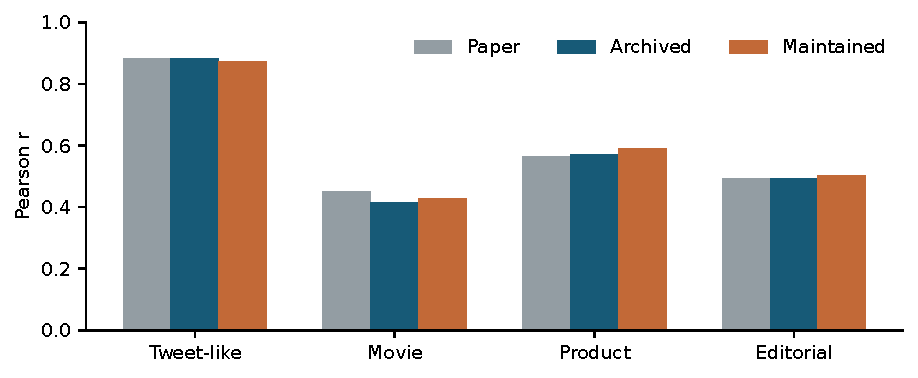
\includegraphics[width=.88\textwidth]{replication_correlations.pdf}
\caption{Reported and reproduced intensity correlations. Maintained code does
not consistently move every collection closer to the original published value.}
\label{fig:replication}
\end{figure*}

The maintained implementation produces correlations of 0.872217, 0.427597,
0.589628 and 0.502898 in the same corpus order. It improves the movie correlation
relative to the archived run, but moves tweet-like and product values further
from their published targets. Therefore, replacing archived code with maintained
code would change the replication question rather than resolve it automatically.

Resource comparison finds 7,502 unique archived lexicon entries and 7,506
maintained entries: four additions, no removals, and two changed valences among
shared entries. The implementations also differ in rule processing. This audit
establishes that version choice matters, but does not isolate the causal effect
of lexicon changes from rule changes. Checksummed inputs and fixed counts reduce
the risk of accidental local substitutions; they cannot establish that the released
artefacts exactly match every intermediate resource used for the original paper.

\subsection{Classification protocol audit}
Under the notebook's provisional policy, archived tweet-like macro-F1 is 0.746696.
This is substantially below the paper's overall F1 of 0.96. The audit evaluates
predefined alternatives for converting the human mean $h$: the notebook policy
$h/4$, the unscaled released mean $h$, and the VADER-style nonlinear mapping
$h/\sqrt{h^2+15}$. Each uses the same fixed class thresholds. Macro and weighted
aggregation are then reported separately.

\begin{table*}[t]
\centering\small
\begin{tabular}{lrrrr}
\toprule
Corpus & $h/4$ macro & $h$ macro & $h$ weighted & Paper F1\\
\midrule
Tweet-like & 0.747 & 0.714 & 0.958 & 0.96 \\
Movie & 0.405 & 0.397 & 0.585 & 0.61 \\
Product & 0.513 & 0.446 & 0.615 & 0.63 \\
Editorial & 0.521 & 0.430 & 0.544 & 0.55 \\
\bottomrule
\end{tabular}

\caption{Archived classification sensitivity. Columns vary reference-score scale
and F1 averaging, not the VADER threshold. The raw-mean/weighted tweet-like value
rounds to 0.96, but this numerical resemblance does not establish the original
evaluation protocol.}
\label{tab:policy}
\end{table*}

The change in neutral support is especially informative. For tweet-like texts,
$h/4$ yields 297 neutral reference items, whereas the unscaled policy yields only
40. Under the latter policy, weighted F1 is 0.957756 and accuracy is 0.940000;
macro-F1 is still only 0.713843. A high weighted score can therefore coexist with
much weaker performance when each class receives equal weight.

The raw-mean/weighted result reproduces the rounded headline F1 numerically, but
does not justify claiming a recovered protocol. The paper describes normalised
thresholds and overall metrics, while these alternative choices produce different
reference partitions. Moreover, the same alternative does not exactly recover
the other collections. The appropriate outcome is an explicit sensitivity result
and an unresolved protocol difference, rather than a claim that the original
research contains an error. No threshold was selected to maximise test scores.

\subsection{Examples from the original data}
Table~\ref{tab:originalexamples} adds qualitative evidence from the released
tweet-like corpus. Items 4 and 35 agree with the derived reference class. Item 266
has a positive human mean but receives zero from both implementations, consistent
with difficulty capturing implicit positive context. For item 431, archived code
returns a positive score despite a negative reference; maintained code returns
a negative score.

\begin{table*}[t]
\centering\small
\begin{tabular}{rlrrrl}
\toprule
ID & Text & Human mean & Archived $c$ & Maintained $c$ & Ref. class\\
\midrule
4 & LMAO, AMAZING! & 2.8571 & +0.8398 & +0.8398 & positive \\
35 & Anger is ugly. & -1.0105 & -0.7906 & -0.7906 & negative \\
266 & Daydreaming about spring. & 1.1789 & +0.0000 & +0.0000 & positive \\
431 & Not a good day & -1.8144 & +0.4404 & -0.3412 & negative \\
\bottomrule
\end{tabular}

\caption{Observed original-data examples. Reference classes use the explicitly
provisional human-mean/4 policy and fixed thresholds. Items were selected after
evaluation to illustrate agreement and disagreement; they do not estimate error
prevalence.}
\label{tab:originalexamples}
\end{table*}

A controlled diagnostic changes only the initial capital in item 431:
``not a good day'' receives $-0.3412$ from both versions. The archived negation
helper checks tokens directly, and this example exposes sensitivity to the
capitalised negator. This post-hoc probe is excluded from aggregate results and
does not by itself explain the remaining corpus-level correlation differences.

\section{Construction and preparation of new data}

\subsection{Existing benchmark: DynaSent}
DynaSent provides English negative, neutral and positive labels. Its first round
contains naturally occurring review sentences; the second contains crowdsourced
adversarial sentences. The creators designed challenging evaluation splits and
validated items with multiple human judgements \citep{potts2021dynasent}. This
project uses the official version 1.1 Round 1 and Round 2 test files, containing
3,600 and 720 sentences respectively. Each split is balanced across the three
classes: 1,200 items per class in Round 1 and 240 in Round 2.

The pinned release revision is \texttt{707b6208}.\footnote{Dataset and datasheet:
\url{https://github.com/cgpotts/dynasent}.}
Parsing checks confirm no empty text, invalid label, duplicate identifier, or
duplicate normalised text within either test split. Normalisation changes only
whitespace, affecting 104 Round 1 strings and 31 Round 2 strings. Case,
punctuation, negation and word order are retained. Stop-word removal or aggressive
regular-expression cleaning would remove signals used by the model.

A minimal data example has fields \texttt{text\_id}, \texttt{sentence} and
\texttt{gold\_label}. One released item, \texttt{r2-0019256}, contains the sentence
``The art exhibit has a lot to offer.'' and a positive reference label.
Reference labels come from the release and are never overwritten by model output.
Official training and development data are not used for model fitting or threshold
selection in this project.

There is one normalised exact-text overlap between Round 1 and the original
corpora, and none for Round 2. The headline benchmark evaluation retains the
official test split and records this overlap. This small overlap qualifies a
claim of complete data independence, even though no classifier training occurs.
The benchmark is also a selected challenge set, so its scores should not be
interpreted as population estimates for all recent English writing.

\subsection{Project route and benchmark role}
The independently chosen VADER paper, code and original corpora form the basis of
the novel project. The supplied overall criteria require replication and newly
created data; they do not impose a first-ever application requirement on each
existing benchmark. DynaSent is used as transfer evidence. Prior work by
\citet{wang2026msra} uses VADER among its weak-supervision sources and evaluates
DynaSent, so this report makes no first-use claim. The 288-text controlled corpus
is the project's newly created data, with human validation still pending.

\subsection{New controlled corpus}
The constructed dataset contains 48 families and 288 unique English texts. Each
family has six conditions: a base sentence, negation, a degree modifier, capitals,
three exclamation marks, and a contrast clause. Four domains contain 12 families
each: apps, transport, university services and customer service. Within each
domain, four base families were drafted to express a positive attitude, four a
negative attitude and four a neutral description.

This targeted design follows the behavioural-testing rationale of
\citet{ribeiro2020checklist}: specific linguistic capabilities are inspected
alongside aggregate performance. The tests are implemented in the project's
own scripts.

The corpus was authored with the ChatGPT/Codex assistant on 4 November 2026.
This provenance is recorded for every item. The base-tone metadata expresses
drafting intentions and is not a human reference label. An intended positive word
can be absent from the lexicon, and a seemingly factual service description can
contain a word with a context-free valence. Such cases were retained rather than
rewritten after seeing predictions.

For example, a family begins with ``The shopping app is frustrating.'' Its
variants include ``not frustrating'', ``extremely frustrating'', an uppercase
sentiment word, exclamation marks and a favourable refund clause after
``but''. Neutral families supply controls: adding capitals to a time or a room
number should not automatically create an emotional assessment. Some neutral
modifier variants adjust descriptive precision rather than sentiment intensity;
their interpretation therefore needs human checking.

The family split was fixed before scoring: twelve families (72 texts) for
development and 36 families (216 texts) for held-out evaluation, with no family
overlap. Model settings remain fixed. Keeping related variants together limits
leakage between partitions; AI authorship and templated wording still limit
generalisability.

\subsection{Independent annotation procedure and status}
Two blank, independently randomised annotation sheets have been prepared.
Readers see an opaque item ID and text, with no design tone, family label,
condition, prediction or other reader's judgement. The protocol requests a class,
an integer intensity from $-4$ to $+4$, confidence and an optional note. A
development pilot precedes the held-out rating. The guidelines distinguish
sentiment from a merely factual event and allow uncertainty about mixed clauses.

After actual independent ratings are collected, raw agreement and Cohen's kappa
\citep{cohen1960agreement} will be computed before discussion. An adjudication sheet will preserve both
original ratings and a final class; unresolved cases will remain ambiguous and
their counts will be reported. Held-out class metrics will use resolved labels.
Intensity agreement will use the mean of the two independent ratings, while
confidence intervals will resample whole families.

\citet{artstein2008agreement} explain how agreement coefficients depend on their
chance model and category distributions. Class counts and raw agreement will
therefore accompany kappa, rather than treating one coefficient as sufficient
evidence of annotation quality.

At the time of this draft, both human rating columns are empty. No human kappa,
constructed-data human accuracy, or correlation with human intensity is available.
The validation script returns a pending status rather than interpreting blank
entries as neutral. Completing this procedure is necessary to answer the third
research question as originally proposed.

\section{Results on new data}

\subsection{Benchmark transfer}
Table~\ref{tab:benchmark} reports the observed benchmark results. Archived macro-F1
is 0.548928 on Round 1 and 0.522994 on Round 2. Maintained values are 0.551640
and 0.522928. Accuracy is 0.561111 and 0.526389 for archived code, and 0.563889
and 0.526389 for maintained code. Both versions exceed the all-neutral baseline
of one-third accuracy and one-sixth macro-F1 on these balanced splits.

\begin{table*}[t]
\centering\small\begin{tabular}{llrrrr}
\toprule
Test split & Version & $n$ & Accuracy & Macro-F1 & 95\% interval\\
\midrule
Round 1 & Archived & 3,600 & 0.5611 & 0.5489 & [0.533, 0.566] \\
Round 1 & Maintained & 3,600 & 0.5639 & 0.5516 & [0.536, 0.568] \\
Round 2 & Archived & 720 & 0.5264 & 0.5230 & [0.485, 0.561] \\
Round 2 & Maintained & 720 & 0.5264 & 0.5229 & [0.485, 0.560] \\
\bottomrule
\end{tabular}

\caption{Observed DynaSent test results. Percentile intervals use 2,000 paired
sentence bootstrap samples with seed 8240. All inputs, labels and thresholds are
fixed; no development-set selection or classifier training is performed.}
\label{tab:benchmark}
\end{table*}

\begin{figure*}[t]
\centering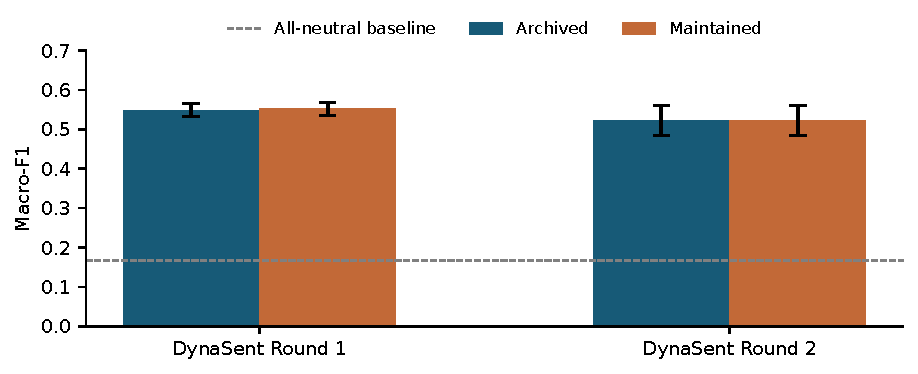
\includegraphics[width=.86\textwidth]{benchmark_f1.pdf}
\caption{Macro-F1 with 95\% bootstrap intervals. The two VADER implementations
have similar performance on each official test split. The baseline predicts
neutral for every item.}
\label{fig:benchmark}
\end{figure*}

The paired maintained-minus-archived macro-F1 interval is $[-0.0022,0.0078]$ for
Round 1 and $[-0.0079,0.0084]$ for Round 2. Both contain zero. The observed
implementation differences are small relative to sampling variation on these
sets, so the results do not support a confident improvement claim for maintained
VADER. The intervals describe resampling uncertainty for the observed test data,
not uncertainty over all possible collection processes.

\citet{dror2018significance} emphasise matching statistical comparisons to the
task, metric and experimental design. Here, paired resampling preserves the
shared test examples when comparing implementations.

Class-specific performance gives more detail than the headline score. Archived
Round 2 negative recall is 0.408, compared with 0.617 for positive items
(Table~\ref{tab:class}). Of 240 negative examples, 87 are predicted positive and
55 neutral. These counts suggest that negative judgements involving context
remain difficult. The confusion pattern also prevents an interpretation in which
the model merely finds the correct sentiment but slightly miscalibrates intensity.

\begin{table}[t]
\centering\small\begin{tabular}{lrrr}
\toprule
Class & Precision & Recall & F1\\
\midrule
Negative & 0.544 & 0.408 & 0.467 \\
Neutral & 0.554 & 0.554 & 0.554 \\
Positive & 0.493 & 0.617 & 0.548 \\
\bottomrule
\end{tabular}

\caption{Archived VADER on DynaSent Round 2. Each reference class has 240 items.}
\label{tab:class}
\end{table}

\begin{figure*}[t]
\centering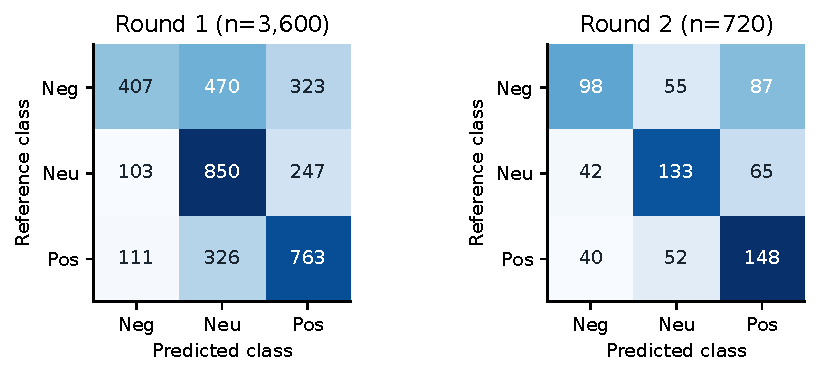
\includegraphics[width=.88\textwidth]{benchmark_confusion.pdf}
\caption{Archived VADER confusion matrices. Rows are released human reference
classes and columns are predictions. Round 1 has many negative items labelled
neutral; Round 2 also has substantial negative-to-positive confusion.}
\label{fig:confusion}
\end{figure*}

These classification results must not be compared numerically with the original
Pearson correlations as if they shared a scale of correctness. Even comparisons
with original provisional macro-F1 require care: the original reference classes
were derived from intensity ratings, whereas DynaSent supplies categorical
labels. Different domains, collection procedures and reference policies can all
contribute to the score change. The experiments show transfer limitations without
identifying any single cause as definitive.

\subsection{Controlled behavioural diagnostics}
Table~\ref{tab:diagnostic} describes archived score changes on held-out families.
Positive-design families move downward under negation by a mean of 0.704;
negative-design families move upward by a mean of 0.688. Modifier, capital and
punctuation conditions generally strengthen the score in the base direction.
Contrast moves the mean toward the newly introduced opposing evaluation.

\begin{table*}[t]
\centering\small\begin{tabular}{lrrrr}
\toprule
Variant & Pos. $\Delta$ & Check & Neg. $\Delta$ & Check\\
\midrule
Negation & -0.704 & 10/12 & +0.688 & 11/12 \\
Modifier & +0.041 & 10/12 & -0.052 & 11/12 \\
Capitals & +0.095 & 10/12 & -0.122 & 11/12 \\
Punctuation & +0.111 & 10/12 & -0.142 & 11/12 \\
Contrast & -0.833 & 12/12 & +0.809 & 12/12 \\
\bottomrule
\end{tabular}

\caption{Held-out constructed diagnostics: mean variant-minus-base compound
change and count satisfying the drafting-direction check. Each tone has 12
families. Checks use AI-authored design hypotheses and are not human accuracy
measurements. Positive and negative refer to intended base tones.}
\label{tab:diagnostic}
\end{table*}

The incomplete direction-check counts are informative. Two positive-design
held-out bases are not strengthened by the intensity variants, while one
negative-design family also fails these checks. For instance, the base about a
reliable delivery team receives a zero archived compound score. By contrast, a
factual help-desk closing-time sentence receives 0.4019, and its negated version
does not express a negative service opinion in the same straightforward way.
The lexicon can activate on a word's context-free association even when the full
sentence is intended as a neutral fact.

\begin{figure*}[t]
\centering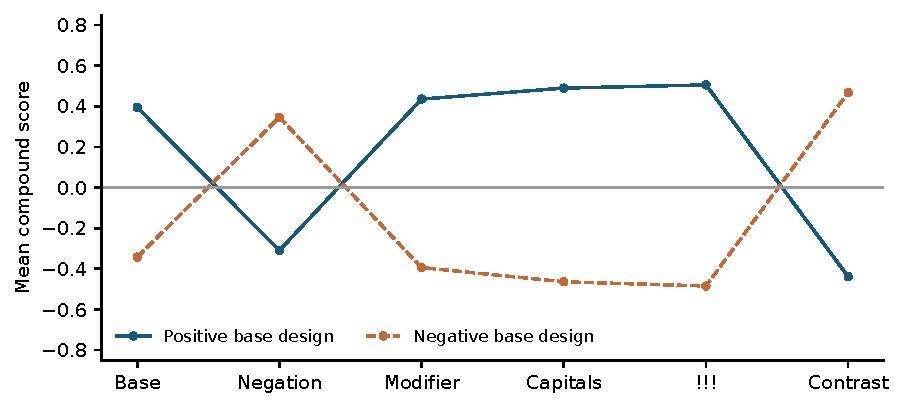
\includegraphics[width=.88\textwidth]{constructed_scores.pdf}
\caption{Archived mean compound scores for the 24 held-out families drafted with
positive or negative base tones. Maintained scores have identical means in this plot.
Lines show numerical model behaviour. Their direction
does not establish agreement with independent human interpretation.}
\label{fig:constructed}
\end{figure*}

The results therefore distinguish rule execution from semantic success. A
punctuation rule cannot intensify a sentiment token that the model never
recognises; an active lexical entry can also induce sentiment in a neutral
description. The 288 inputs and their predictions make these cases inspectable,
but assigning a human-correctness score requires the outstanding reference
ratings. The examples are qualitative illustrations selected after scoring, so
they do not estimate the prevalence of each failure type in natural language.

\subsection{LLM-as-judge pilot}
The evaluation includes two 60-item within-session assistant judgements. The
DynaSent sample contains 20 items from each released gold class, selected with
seed 8240. The constructed sample contains all six variants from ten held-out
families. Judge-input files contain IDs and texts, while labels, VADER scores
and condition names are omitted. The prompt requests one class, a supporting
phrase, confidence and a brief explanation per item.

The judge was the ChatGPT/Codex assistant in the current conversation. The
interface did not expose an exact serving-model snapshot, temperature or decoding
seed. It was not an external API experiment. Inputs, responses, prompt and
provenance limitations are preserved, allowing exact rescoring of the recorded
outputs. Re-running a closed model to regenerate identical outputs is a separate
and unresolved reproducibility problem.

\begin{table}[t]
\centering\small\begin{tabular}{lrr}
\toprule
System on the same 60 items & Accuracy & Macro-F1\\
\midrule
Archived VADER & 0.500 & 0.498 \\
Maintained VADER & 0.483 & 0.484 \\
Assistant judge & 0.883 & 0.883 \\
\bottomrule
\end{tabular}

\caption{Exploratory comparison on the same balanced 60-item DynaSent sample.
The assistant result comes from preserved within-session textual judgements.}
\label{tab:judge}
\end{table}

On the sampled DynaSent items, the assistant agrees with the released human class
in 53 of 60 cases: accuracy 0.883333, macro-F1 0.882784 and kappa 0.825.
Archived VADER has macro-F1 0.498074 on these same items. The judge macro-F1
bootstrap interval is $[0.792,0.952]$. This small exploratory comparison is
consistent with useful contextual interpretation, but supports no broad claim
that the assistant replaces human annotation.

The seven judge mismatches include ambiguous fragments and differences between
inferred event valence and the dataset's overall sentiment label. For example,
the judge treats a threatening action as negative while the released item is
neutral. A fragment is assigned neutral despite a positive released label.
These differences illustrate why a plausible explanation is not a substitute
for agreement with a declared reference policy.

On the constructed sample, archived and maintained VADER each agree with the
assistant on 44 of 60 labels (0.733333). This is model-to-model agreement only.
The assistant also authored the constructed corpus and retained broader
conversation context. Thus the constructed trial is not independently blinded,
and shared authorship may make the examples easier for the judge.
\citet{liu2023geval} motivate structured model-based assessment and identify
potential evaluator bias, but their generation-quality experiments do not validate
this sentiment-classification adaptation. Comparison with actual constructed-data
human labels remains pending.

\section{Ethical considerations}

\subsection{Data, participation and attribution}
The Australian Code emphasises responsible research practice, transparent
reporting, proper acknowledgement and sound handling of research information
\citep{researchCode}. Applied here, these principles require clear data provenance,
preservation of unfavourable results, separation of evidence from plans, and
accurate attribution of reused code and annotations. A failed or incomplete
replication is reported as such rather than repaired through undisclosed changes.

Documenting the constructed corpus's motivation, composition, creation process
and intended uses follows the transparency rationale of
\citet{gebru2021datasheets}. Its manifest and annotation guidelines record these
properties and the outstanding human-validation limitation.

The original study used crowdsourced judgements. Their quality-control methods
and aggregated references are part of the published study, but this project does
not establish new consent or review the original recruitment. The replication
uses the released artefacts and avoids re-identifying authors of the adapted
texts. Public availability is treated as a source-access property rather than
automatic permission for unrestricted redistribution.

The upstream VADER code includes an MIT notice, which is retained. DynaSent's
repository and datasheet discuss its release and potential inherited Yelp terms
\citep{dynasentData}. The public project should distribute retrieval instructions,
IDs and derived scores rather than a replacement copy of the full source
collections. The local judge input records contain a small evaluation sample;
publication of those texts should follow the source conditions. No API keys or
credentials belong in the report or repository.

The proposed new annotation uses volunteers. Actual participation should follow
course guidance, with informed agreement, freedom to stop and no unnecessary
personal information in public files. Anonymous reader codes are sufficient for
the computational audit. Consent records and contact details should remain
private. No institutional ethics approval or completed recruitment is claimed in
this report.

\subsection{Model bias and interpretation}
VADER's lexicon and rules represent particular language and rating conventions.
An English short-text evaluation does not establish reliability for other
languages, dialects, groups or specialised decisions. The constructed corpus
covers only four service-related domains and a restricted set of sentence forms.
AI-assisted drafting can add stereotyped wording and favour examples that match
the drafter's own interpretation. Maintaining negative, neutral and ambiguous
cases reduces selective reporting, while independent annotation is needed to
test these assumptions.

Sentiment output should also be interpreted at the appropriate level. A label
about a review sentence does not establish the writer's psychological state,
intent, trustworthiness or future behaviour. The false positives in factual
service descriptions make such inferences particularly weak. The present
evaluation supports analysis of declared text-level sentiment tasks rather than
individual profiling or consequential automated decisions.

The assistant judge adds a different source of bias. Its training-data overlap
with a known public benchmark cannot be excluded, and the current interface does
not provide the controls needed for an independently repeatable model trial.
Its explanations may be persuasive even where its label disagrees with the
reference. Keeping human gold unchanged, recording low-confidence judgements
and reporting mismatches limits the risk of treating fluency as correctness.

\subsection{Research integrity and AI assistance}
Generative AI assisted corpus drafting, software preparation, the textual judge
pilot and report writing. Computational values in the report are exported from
executed scripts and preserved result files. Authorship provenance and judge
limitations are disclosed. Human annotation was not simulated, and missing
measurements are not replaced by estimates presented as observations.

The student remains responsible for checking the source papers, interpreting the
results and verifying the submitted text under the assessment's open-AI policy.
The unchanged Assessment 1 and 2 files remain background evidence; their planned
work is not automatically described as completed. The DynaSent novelty claim was
revised when contrary evidence was found. These choices keep the final argument
consistent with the available experimental record.

\section{Conclusions and reflections}
Archived VADER can be executed successfully on all released original texts, and
two of the four published correlations reproduce to three decimal places.
Movie and product values differ, while maintained code changes performance
without resolving every discrepancy. The classification audit demonstrates that
reference-score conversion and F1 averaging materially affect conclusions.
A rounded headline match under one alternative policy is insufficient to establish
full replication of the original protocol.

On the official DynaSent tests, both implementations achieve similar macro-F1,
around 0.55 in Round 1 and 0.52 in Round 2. They exceed a constant-class baseline
but retain substantial class-specific errors. This is evidence of limited
transfer under fixed settings. It does not imply a general score for all modern
short text or isolate domain shift as the only cause of failure.

The constructed corpus provides an inspectable set of 288 related inputs and
reveals interactions between lexical coverage and contextual rules. The
within-session judge pilot offers additional exploratory interpretation, with
preserved outputs and explicit reproducibility limits. Independent human
annotation of the constructed texts remains the main unfinished scientific
dependency. Completing it will permit kappa, human-reference class metrics,
intensity correlation and paired family-level analysis, answering the third
research question on its intended basis.

Data identity, reference policy, version selection and the distinction between
human and model judgement determine which conclusions the numbers can support.
The supplied scripts make these decisions auditable.

\clearpage
\balance
\bibliography{references}
\end{document}
